\section{Basic Electronic Components}


The following sections briefly introduce electronic components. Each of these pieces can be used to make complex, powerful circuits.\footnote{Most of these definitions come from Wikipedia, though they have been edited and augmented by the author in several places.}

\subsection*{Resistors} 

A resistor limits the electrical current that flows through a circuit. Resistance is the restriction of current. In a resistor, the energy of the electrons that pass through the resistor are changed to heat and/or light. For example, in a light bulb there is a resistor made of tungsten which converts the electrons into light and a great deal of heat.

\begin{center}
  	\begin{circuitikz}
    	\draw (0,0)
      	to[battery] (0,2) % 
     	to[R=$R_1$] (2,2)
     	to[short] (2,0) -- (0,0) 
		;

     	\draw (0,0)
      	node[ground] {} % ground connection
		;
		\node[scale=0.7, thick ] at (-0.25,1.4) {$+$};
		\node[scale=0.7, thick ] at (-0.25,0.6) {$-$};

   \end{circuitikz}

{A very simple circuit. Electricity flows through the resistor (maybe it's a light bulb). The resistor controls how much current flows in the circuit, and heats up.}
\end{center}



\subsection*{Capacitors}

A capacitor (also called condenser, which is the older term) is an electronic device that stores electric energy (a ``charge''). It is similar to a battery, but is smaller, lightweight and charges up much quicker. Typically, capacitors hold much less energy than a battery, but can provide almost their entire charge to the circuit quickly. Capacitors are used in many electronic devices today, and can be made out of many different types of material. 

The Leyden jar was one of the first capacitors invented: metal foil was placed inside a glass jar, and wrapped around the outside of a glass jar, but neither foil gets near the top of the jar. The glass barrier between the foil sheets (inside and outside) allows a charge to build up between the foil without allowing the electrical charge to move through the glass. Leyden jars didn't hold much charge, but the concept it demonstrated has not changed.

Capacitors are usually made with two metal plates that are on top of each other (or wrapped around each other), but that do not actually touch. When powered, they allow energy to be stored inside an electrical field. Because the plates need a lot of area to store even a small amount of charge, the plates are usually rolled up into some other shape, such as a cylinder. Sometimes, other shapes of capacitors are used for special purposes. A capacitor-like effect can also result just from two conductors being close to each other, whether you want it to exist or not-- if you've ever been shocked by a door knob or metal refrigerator in the winter, you have been one plate of a capacitor, because you've been storing a charge!

\begin{center}
  	\begin{circuitikz}
    	\draw (0,0)
      	to[battery] (0,2) % 
     	to[C=$C_1$] (2,2)
     	to[short] (2,0) -- (0,0) 
		;

     	\draw (0,0)
      	node[ground] {} % ground connection
		;
		\node[scale=0.7, thick ] at (-0.25,1.4) {$+$};
		\node[scale=0.7, thick ] at (-0.25,0.6) {$-$};

		\vertionarray{0.75}{2}{\ionradius}{$+$}
		\vertionarray{1.25}{2}{\ionradius}{$-$}
   \end{circuitikz}

\medskip
\end{center}
{Open capacitors in a steady state. No current flows, but there is a charge.}


\bigskip
\stbox{
\emph{Experiment:} make a variable capacitor from aluminum foil, paper, and a paper towel tube. The paper should go around the roll only once. Cut the foil one-quarter or one-half inch smaller than the paper on all sides. Tape a small wire to one corner of the foil, if possible using metallic/conductive tape\footnote{See the appendices for guidance on soldering to aluminum foil}. Tape the foil to the paper. Tape one edge of the paper, foil side down, against the cardboard tube. Make another paper/foil combination. Wrap the paper/foil around the cardboard tube, but tape the paper only to itself, and just loose enough to slide a little. 

\bigskip

It is also possible to make a regular capacitor with the paper-foil layers, separated by flat sheets of cardboard. Keep track of the ``up'' and ``down'' sides! Note that it is pretty easy to gang each ``plate'' together and make capacitor with a larger value; tying all the anodes together, and all the cathodes together, makes a larger capacitor.
}

\subsection*{Diodes}

A diode is an electronic component with two electrodes (connectors). It allows electricity to go through it only in one direction.

Diodes can be used to convert alternating current to direct current (this circuit is called a diode bridge). They are often used in power supplies and can be used to decode AM (``amplitude modulation") radio signals (like in a crystal radio). Light-emitting diodes (LEDs) are a type of diode that produce light. 


\begin{center}
  	\begin{circuitikz}
    	\draw (0,0)
      	to[battery] (0,2) % 
     	to[R=$R_1$] (2,2)
		to[empty led](2,0)
     	to[short] (2,0) -- (0,0) 
		;

		\draw(2.5, 1.5)
		node[right]{$D_1$};

     	\draw (0,0)
      	node[ground] {} % ground connection
		;
		\node[scale=0.7, thick ] at (-0.25,1.4) {$+$};
		\node[scale=0.7, thick ] at (-0.25,0.6) {$-$};

   \end{circuitikz}

\medskip
\end{center}

{A very simple circuit. Electricity flows through the resistor, that controls how much current flows into the LED. If the battery was put in backwards,  no electricity could flow in the opposite direction, so the LED would not light up.}


\subsection*{Inductors (Coils)}

An inductor, also called a coil or (rarely) a reactor, is a two-terminal electrical component that stores electrical energy in a magnetic field, when electric current is flowing through it. An inductor typically consists of an electric conductor, such as a wire, that is wound into a \emph{coil}. Sometimes inductors include a magnetic bar or ring, around which the wire is wound. Other times the wire is wound with only air in the middle (which still works, because the Earth has a magnetic field).

Inductors do many interesting things. For instance, they are used to block AC while allowing DC to pass; inductors designed for this purpose are called \emph{chokes}. They are also used in electronic filters to separate signals of different frequencies, and in combination with capacitors to make tuned circuits, used to tune radio and TV receivers.

\noindent The symbol for an inductor is a coil icon. Inductors are usually abbreviated with an L: 

\bigskip

\begin{center}
  	\begin{circuitikz}
    	\draw (0,0)
      	to[battery] (0,2) % 
     	to[L, l^=$L_1$] (2,2) % The inductor
		to[C, l^=$C_1$](2,0)
     	to[short] (2,0) -- (0,0) 
		;

     	\draw (0,0)
      	node[ground] {} % ground connection
		;
		\node[scale=0.7, thick ] at (-0.25,1.4) {$+$};
		\node[scale=0.7, thick ] at (-0.25,0.6) {$-$};

   \end{circuitikz}

\medskip
\end{center}

A simple circuit with one coil and one capacitor. This sort of circuit is one way to make an \emph{oscillator}. This kind of circuit is found in radios.


\subsection*{Transistors}

A transistor is a \emph{semiconductor} (see below) device used to amplify or switch electronic signals and electrical power. It is composed of semiconductor material usually with at least three terminals for connection to an external circuit. A voltage or current applied to one pair of the transistor's terminals controls the current through another pair of terminals. Because the controlled (output) power can be higher than the controlling (input) power, a transistor can amplify a signal. Today, some transistors are packaged individually, but many more are found embedded in integrated circuits.

The transistor is the fundamental building block of modern electronic devices. It might be the most important -- or at least the most influential -- engineering discovery, ever.

Why are transistors important? They enable a lot of powerful new devices. 

\bi

\+ They can act like switches -- with no moving parts, and that can be controlled with a tiny electrical signal

\+ They can take a small signal and turn it into a powerful signal; they can make sound louder, broadcast radio signals farther, or detect very tiny changes in other materials (thus, you can have electronic thermometers, or radio telescopes)

\+ When combined into logic gates (more on that below), they enable super-fast computations that have also changed how we do work, science, medicine, and almost every form of research

\ei

\subsection*{A Little History}

Many years ago, a ``computer'' meant ``the person who did the math problems." A few people invented adding machines like an abacus, and \emph{slide rules} made even difficult calculations very possible, but they still required a person to do the math. In the same way, people had learned about electricity, but couldn't do much with it except power light bulbs, street cars, and telegraphs. Talking to someone many miles away meant either using Morse code, or writing a letter. 

\begin{figure}[h!]
\begin{center}
\fbox{
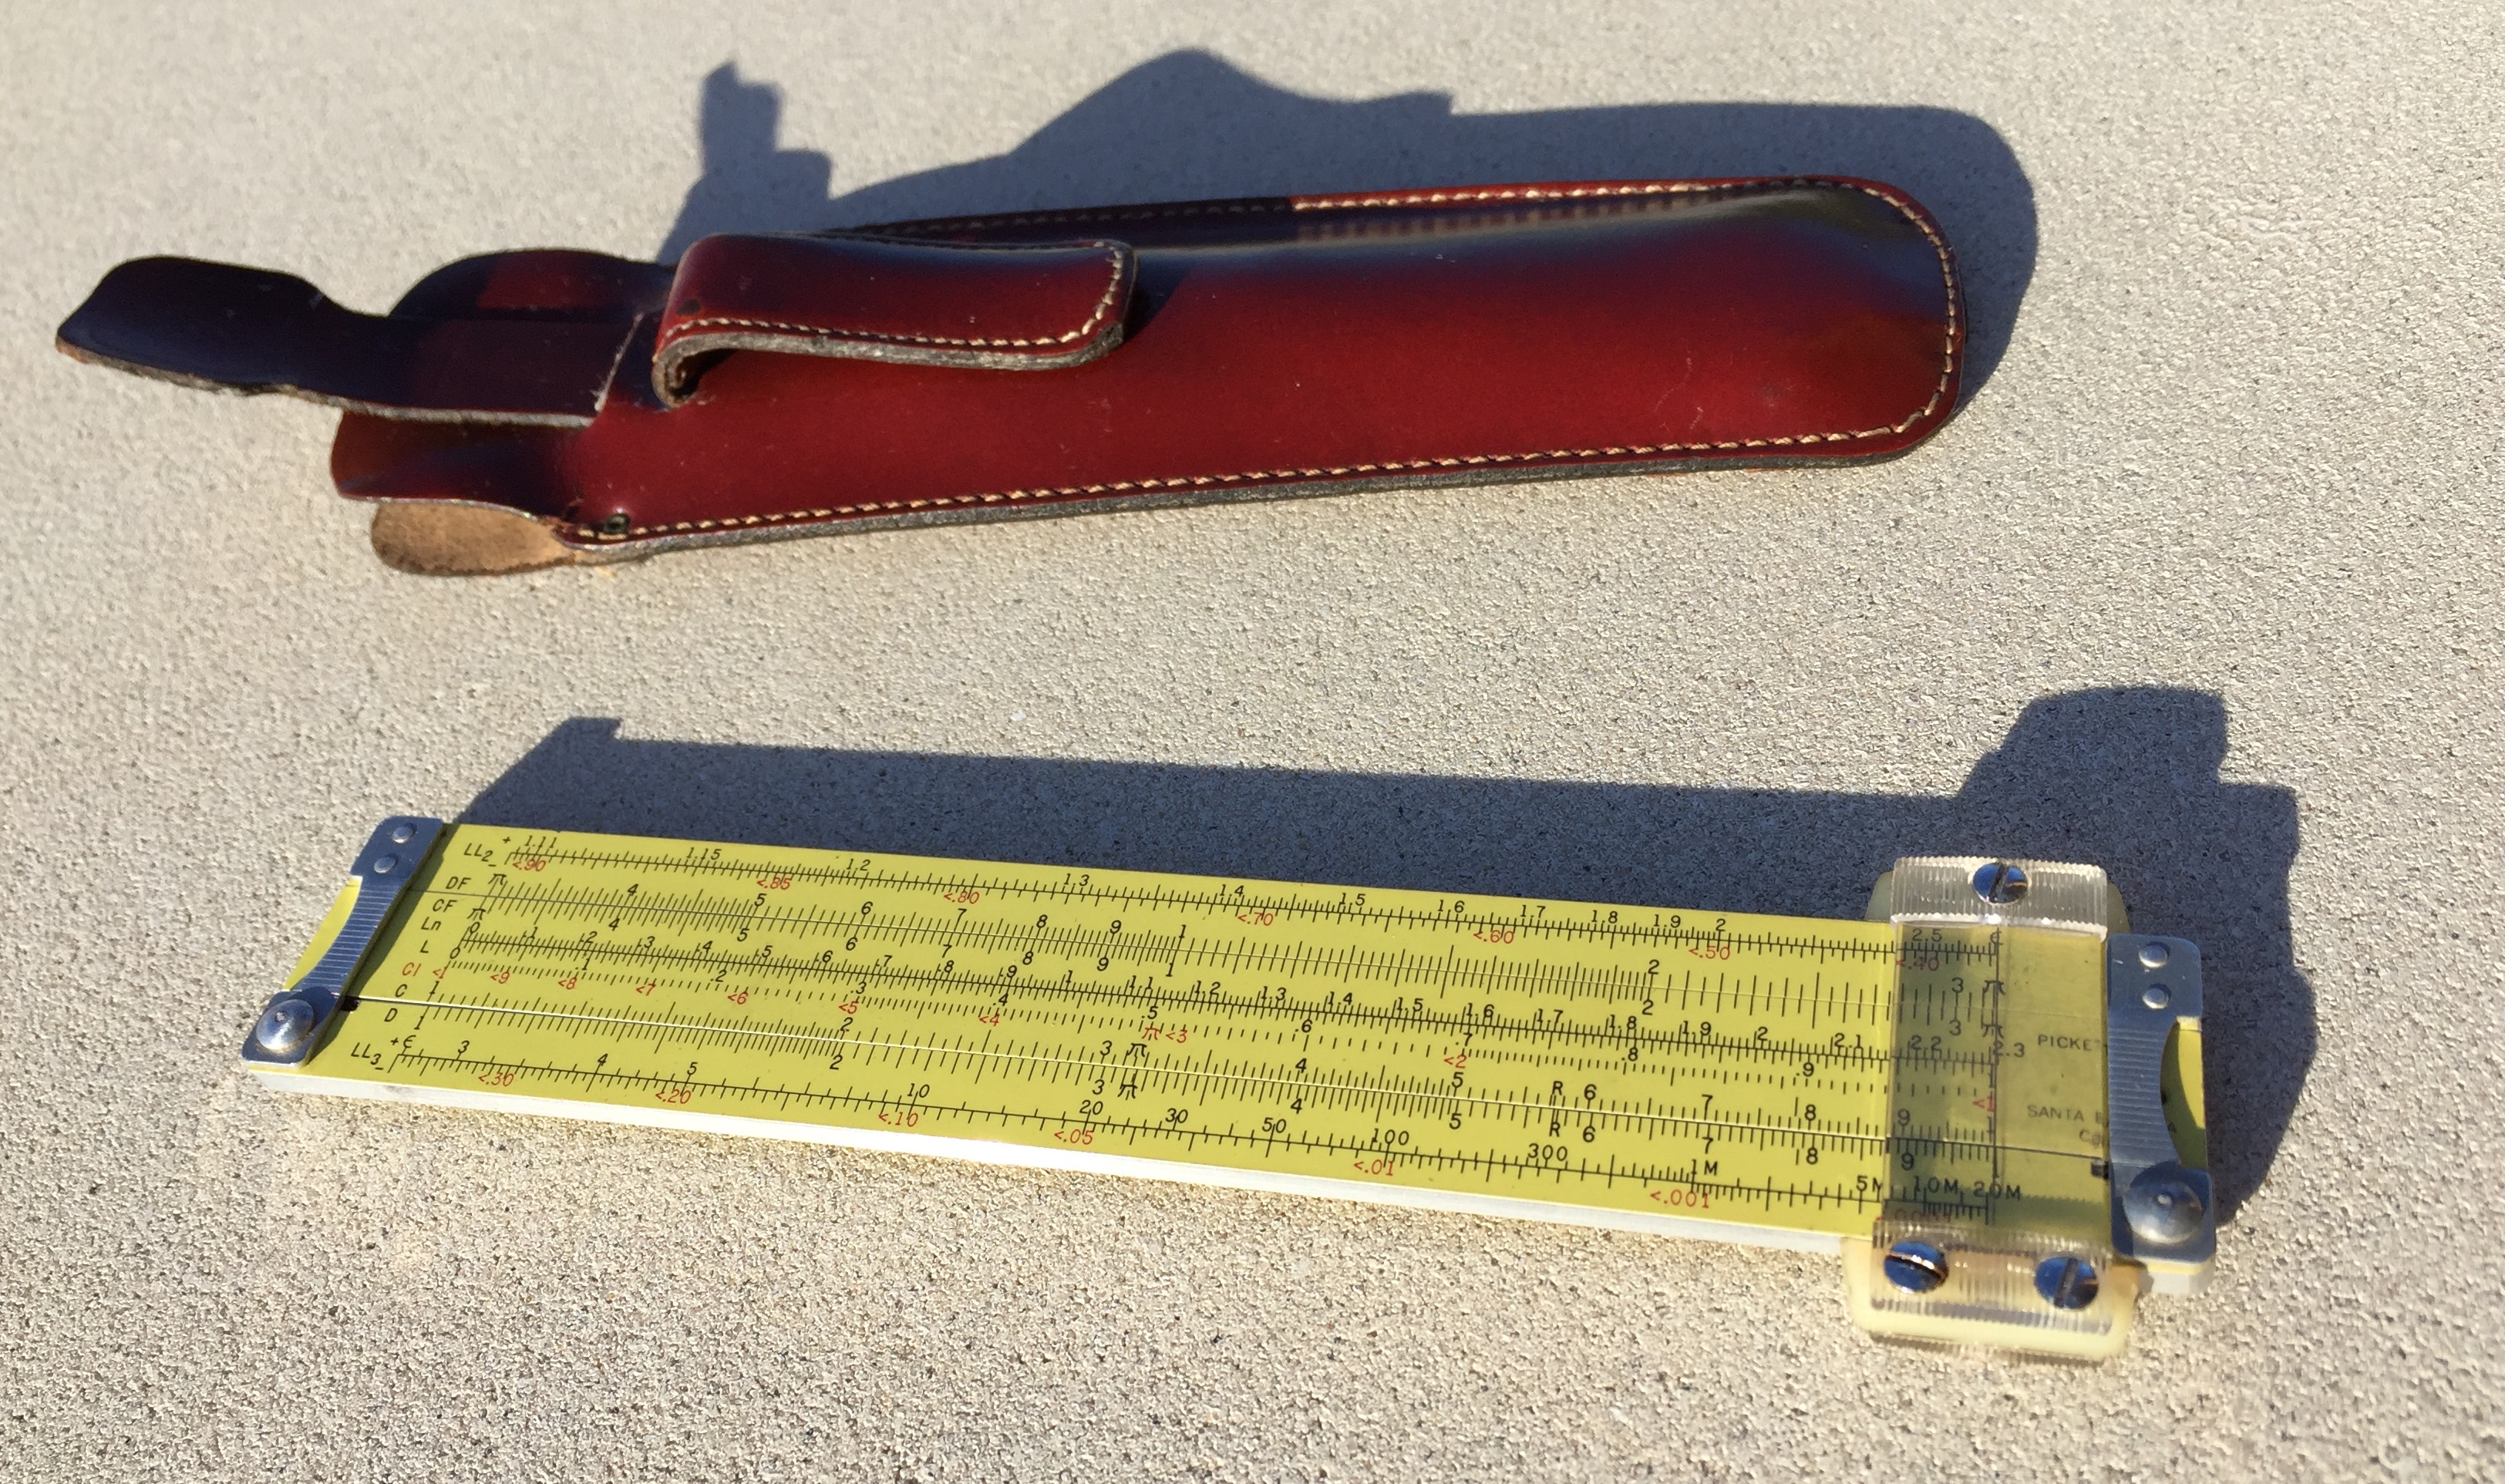
\includegraphics[scale=0.10]{SlideRule-2.jpg}
}
\end{center}
\caption{A pocket-sized slide rule from the late 1960s. This example is one of many that were given as promotional gifts to people who worked on NASA's lunar missions.}
\label{fig:sliderule}
\end{figure}

The first discovery that led to the transistor was the \emph{vacuum tube diode}, which uses a hot wire in a glass enclosure with no air in it to push electrons to another conductor, just like any other diode. Unfortunately, vacuum tube diodes are big, fragile, hard to make, and produce a huge amount of heat. The \emph{vacuum tube triode}, which does everything a transistor does, came next. Since electrons are negatively charged, a slight negative charge on the third wire (between, but not touching, the hot-wire emitter and the collector) permitted people to control the flow of electrons from one side to the other -- it acted like a switch. 

Vacuum tube triodes have all the same shortcomings as the vacuum diode, and have even more parts to fail. Despite their shortcomings, vacuum tubes changed the world in a \emph{huge} way: they enabled radios, televisions, radar, and the first digital computers. But these computers were the size of a small house, weighed 30 tons, and required powerful cooling.

In the 1940s, three scientists discovered that some substances could either behave like an insulator \emph{or} a conductor, depending on how much electricity or heat was applied to it. Being able to change a slab of glass or silicon from an insulator into a conductor meant they could do everything a vacuum tube could do, except much smaller, cheaper, and cooler. About nine years after they announced the discovery and proved that it works, the three men won the Nobel Prize. They had discovered a \emph{semiconductor}. 

\stbox{There's a longer documentary about the transistor on YouTube {\color{webblue}\href{https://www.youtube.com/watch?v=jYxf3gYUZBM}{here}}.}

The world changed amazingly quickly when we started using transistors. Today, there are many different kinds of transistors. The computer in your house has many \emph{billions} of transistors inside it. So does your phone, your car, your microwave, your television...wow!

Some transistors are made especially for certain applications, like making audio louder, or pushing radio signals, or just for doing computations. These are all transistors, but they are different. 




\subsection*{Electronics and Transistors}

Transistors are usually abbreviated with $Q$. There are several kinds of transistors, but they work mostly the same. 

\begin{center}
\begin{circuitikz}
\draw
(1,1) node[npn](Q1){}
(0.5,1.5) node[left](){$Q_1$}
(Q1.B) node[left] {$Base$} %label
(Q1.C) node[right] {$Collector$} %label
(Q1.E) node[right] {$Emitter$} %label
;
\end{circuitikz}
\medskip

Most transistors have three pins. For this kind of transistor (called an ``NPN"):
\bi
\+ Electricity comes in the \emph{collector}
\+ Electricity applied to the \emph{base} opens up the flow of electricity to the \emph{emitter}
\+ Electricity, when able, flows out the emitter and towards a ground.
\+ Therefore, the base is like a switch. It turns the transistor from an insulator into a conductive wire. 
\ei

\end{center}

\noindent Most computers use a transistor type called a ``FET" (\emph{Field Effect Transistor}), that is very efficient and does not require very much electricity to switch from ``on'' to ``off''. They are faster and run cooler than the older types of transistors. Somewhat confusingly, these transistors have different names for their pins, compared to the older ``BJT" type transistors, seen above.

\begin{center}
\begin{circuitikz}
\draw
(1,1) node[nigfete,solderdot](Q2){} % an N-type IGFET, also called a MOSFET
(0.75,1.75) node[left](){$Q_2$}
(Q1.B) node[left](){$Gate$} %label
(Q1.C) node[right]() {$Source$} %label
(Q1.E) node[right]() {$Drain$} %label
;
\end{circuitikz}
\end{center}
\medskip



For questions of computers, we will treat transistors like a switch and nothing more. That's easy, right?

But how do transistors do all the cool stuff they do? Why are pocket calculators or iPhones possible? How do collections of electronic components enable us to do math, send text messages, or simulate a nuclear explosion without anything going kaboom?

At the absolute base of the entire electronics world, just above transistors, are \emph{logic gates}. They are the simplest building blocks of digital computers. 

\stbox{A good additional introduction video is {\color{webblue}\href{http://ed.ted.com/lessons/how-transistors-work-gokul-j-krishnan}{here}} (\texttt{ed.ted.com}).}

